\section{Workflow}\label{sec:workflow}

\Cref{lst:ols} fits ordinary least squares once and attaches two
heteroskedasticity-consistent covariance procedures
\citep{white-1980,mackinnon-white-1985} to the retained fit.

\lstinputlisting[float=t,caption={Two covariance procedures on one retained
fit.},label={lst:ols}]{listings/ols.py}

The coefficients do not change with the covariance procedure. Here the slope
estimate is \jcnum{ols-hc3-x-estimate} under both, while its standard error
is \jcnum{ols-hc0-x-se} under HC0 and \jcnum{ols-hc3-x-se} under
HC3. The normal reference behind the 95\% interval
$[\jcnum{ols-hc3-x-lower}, \jcnum{ols-hc3-x-upper}]$ is chosen explicitly
when the report is formed. Requesting a covariance does not select a reference
distribution, and \texttt{report} computes no default $p$-values. Replacing
HC0 with HC3 changes the uncertainty estimate, but it is not a new point
estimator, and neither procedure is thereby shown to have accurate
finite-sample coverage (\cref{sec:coverage}).

\Cref{lst:poisson} carries a Poisson regression with exposure from fitting to
publication outputs. Given arrays \texttt{load}, \texttt{hours} and
\texttt{incidents} for \jcnum{poisson-n-observations} facilities, the model sets
$\log \mu_i = \beta_0 + \beta_1 \mathrm{load}_i + \log \mathrm{hours}_i$, so
exposure enters with coefficient one rather than as an estimated regressor.
STATADIC supports model-based, HC0 and HC1 covariance for this family and rejects
HC2 and HC3.

\lstinputlisting[float=t,caption={From a Poisson fit to publication outputs.},
label={lst:poisson}]{listings/poisson.py}

The model is fitted directly from a mapping of named arrays; eager Arrow,
Polars and pandas tables are accepted in the same position. Only the declared
roles are read, and explicit 64-bit inputs are rejected rather than narrowed
when JAX's 64-bit mode is off. Each prediction kind requires only the roles it
uses. The expected count needs the exposure, but the rate per unit of exposure
does not, so the listing predicts it from \texttt{load} alone.

The listing produces three kinds of output, each with a deliberately narrow
capability:
\begin{itemize}
  \item \texttt{Report} retains unrounded estimates, availability states,
    metrics and metadata. It renders them as text, HTML or a LaTeX tabular
    without refitting. \Cref{tab:poisson} is that tabular, included unchanged:
    columns that no row populates are omitted, numbers are set in math mode, a
    visible note states the confidence level, reference distribution and
    covariance, and the remaining metadata are kept as TeX comments.
  \item \texttt{PlotSpec} retains precomputed coordinates and renders them
    through Matplotlib or as native PGFplots source.
    \texttt{prediction\_line} evaluates the fitted predictor on the grid and
    retains the resulting coordinates without computing anything else.
    \Cref{fig:rate} is the PGFplots source, included unchanged. Because
    PGFplots keeps axes and coordinates in TeX, the manuscript controls
    typography and styling.
  \item \texttt{fit.save\_predictor} writes a prediction artifact: a JSON
    manifest with schema version \jcvalue{artifact-schema-version} and a
    checksummed little-endian payload of \jcvalue{artifact-payload-bytes}
    bytes for the two coefficients.
\end{itemize}

\begin{table}[t]
  \centering
  \small
  \caption{The HC1 inference report of \cref{lst:poisson}, rendered by
  \texttt{Report.to\_latex} and included unchanged.}
  \label{tab:poisson}
  % Regression inference
\begin{tabular}{@{}lS[table-format=-1.4,group-digits=integer]S[table-format=1.5,group-digits=integer]S[table-format=-1.4,group-digits=integer]S[table-format=-1.4,group-digits=integer]@{}}
\toprule
Parameter & {Estimate} & {SE} & \multicolumn{2}{c}{95\% CI} \\
\cmidrule(lr){4-5}
 & & & {Lower} & {Upper} \\
\midrule
intercept & -0.4942 & 0.06076 & -0.6133 & -0.3751 \\
load & 0.2998 & 0.01636 & 0.2677 & 0.3319 \\
\midrule
n\_observations & {\num{400}} & & & \\
\bottomrule
\end{tabular}
\par 95\% intervals; normal reference; covariance HC1
% {"confidence": 0.95, "covariance": "HC", "covariance_options": {"finite_sample_correction": 1.0, "kind": "HC1"}, "degrees_of_freedom": null, "finite_reference_outside_validated_range": false, "inference_columns": {}, "inference_status": "AVAILABLE", "interval_status": "AVAILABLE", "n_observations": 400, "reference": "normal", "rows": {"count": 400, "sha256": "61c7e6234e65fb5cce2355ea19e2867337eab0f6ef7092bc7e646da03f05ab8e"}}

\end{table}

Loading the artifact restores only the capability
\texttt{\jcvalue{artifact-capabilities}}, with the fitted design and the
exposure role. Its expected counts and rates on new rows match the live fit's,
with a maximum absolute difference of \jcnum{artifact-prediction-difference},
but it does not restore covariance, identification evidence or inference. An
analysis snapshot likewise restores only
\texttt{\jcvalue{snapshot-capabilities}}, and re-rendering it reproduces the
original LaTeX exactly. Plot labels written as raw TeX are refused on loading
unless the caller declares the snapshot trusted. Neither artifact uses Python
object serialization.

\begin{figure}[t]
  \centering
  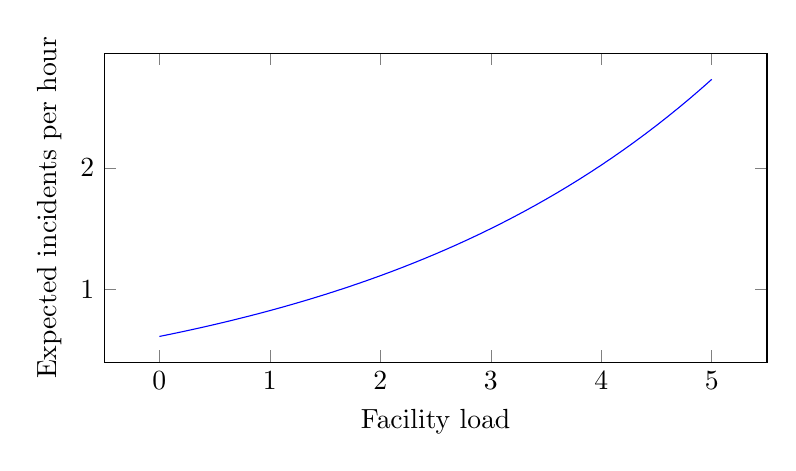
\begin{tikzpicture}
\begin{axis}[width=10cm,height=5.5cm,xlabel={Facility load},ylabel={Expected incidents per hour}]
\addplot+[no marks,forget plot] coordinates {(0,0.6100347203462378) (0.1,0.6286006360560655) (0.2,0.6477315904672131) (0.30000000000000004,0.6674447800777674) (0.4,0.6877579247473941) (0.5,0.7086892836254246) (0.6000000000000001,0.7302576715637046) (0.7000000000000001,0.7524824760289517) (0.8,0.7753836745298284) (0.9,0.7989818525743939) (1,0.8232982221740766) (1.1,0.8483546409107994) (1.2000000000000002,0.8741736315843982) (1.3,0.9007784024579943) (1.4000000000000001,0.9281928681195168) (1.5,0.95644167097813) (1.6,0.9855502034148875) (1.7000000000000002,1.015544630607522) (1.8,1.0464519140498907) (1.9000000000000001,1.0782998357872162) (2,1.1111170233889054) (2.1,1.144932975681399) (2.2,1.1797780892641774) (2.3000000000000003,1.2156836858327602) (2.4000000000000004,1.2526820403332606) (2.5,1.2908064099737988) (2.6,1.3300910641188561) (2.7,1.3705713150934402) (2.8000000000000003,1.4122835499247464) (2.9000000000000004,1.455265263049857) (3,1.4995550900188679) (3.1,1.5451928422237455) (3.2,1.5922195426841272) (3.3000000000000003,1.640677462922234) (3.4000000000000004,1.6906101609600437) (3.5,1.7420625204728717) (3.6,1.7950807911345688) (3.7,1.8497126301905813) (3.8000000000000003,1.9060071452962637) (3.9000000000000004,1.9640149386589354) (4,2.0237881525233665) (4.1000000000000005,2.0853805160415795) (4.2,2.148847393569092) (4.3,2.2142458344310203) (4.4,2.281634624202775) (4.5,2.3510743375514354) (4.6000000000000005,2.4226273926853215) (4.7,2.496358107460682) (4.800000000000001,2.5723327571959542) (4.9,2.650619634245547) (5,2.7312891093867098)};
\end{axis}
\end{tikzpicture}

  \caption{Fitted Poisson incident rate per hour of exposure, built by
    \texttt{prediction\_line} and rendered by \texttt{PlotSpec.to\_pgfplots}
    in \cref{lst:poisson}. The estimated slope is
    \jcnum{poisson-load-estimate}, with an HC1 standard error of
  \jcnum{poisson-load-se}.}
  \label{fig:rate}
\end{figure}
